% ----------------------------- %
% Author Guidelines
% ----------------------------- %
\section*{General Guidelines}
\noindent Please read these instructions carefully.   The objective of this template is to enable you in an easy way to style your article attractively in a style similar to that of the typeset journal. It should be emphasized, however, that the final appearance of your paper in print and in electronic media may likely vary to some extent from the presentation achieved in this template.

    \begin{tcolorbox}[breakable, size=fbox, boxrule=1pt, pad at break*=1mm,colback=cellbackground, colframe=cellborder]
\prompt{In}{incolor}{3}{\boxspacing}
\begin{Verbatim}[commandchars=\\\{\}]
\PY{c+c1}{\PYZsh{} I\PYZsq{}m from South Korea, but I grew up in Dubai.}
\PY{n+nb}{print}\PY{p}{(}\PY{l+s+s1}{\PYZsq{}}\PY{l+s+s1}{Hello, my name is: Soobin Rho}\PY{l+s+s1}{\PYZsq{}}\PY{p}{)}
\end{Verbatim}
\end{tcolorbox}

    \begin{Verbatim}[commandchars=\\\{\}]
Hello, my name is: Soobin Rho
    \end{Verbatim}



    
% ----------------------------- %
% Heading Levels
% ----------------------------- %
\subsection*{Level Headings: Subsections}
\noindent You will usually want to divide your article into (numbered) sections and subsections (perhaps even subsubsections).  Use to help organize your document as appropriate. Include hyperlinks using  URL \url{http://www.google.com}.  

Hi! This is for my \inlinecode{Math 125} class.
\pagebreak
    \begin{tcolorbox}[breakable, size=fbox, boxrule=1pt, pad at break*=1mm,colback=cellbackground, colframe=cellborder]
	\prompt{In}{incolor}{9}{\boxspacing}
	\begin{Verbatim}[commandchars=\\\{\}]
		\PY{l+s+sd}{\PYZsq{}\PYZsq{}\PYZsq{}Generates a random sentence.\PYZsq{}\PYZsq{}\PYZsq{}}
		\PY{k+kn}{from} \PY{n+nn}{random} \PY{k+kn}{import} \PY{n}{randint}
		
		\PY{k}{def} \PY{n+nf}{generate\PYZus{}random\PYZus{}sentence}\PY{p}{(}\PY{p}{)} \PY{o}{\PYZhy{}}\PY{o}{\PYZgt{}} \PY{n+nb}{str}\PY{p}{:}
		\PY{l+s+sd}{\PYZsq{}\PYZsq{}\PYZsq{}}
		\PY{l+s+sd}{        1. Picks an article and capitalizes the first letter.}
		\PY{l+s+sd}{        2. Picks a noun.}
		\PY{l+s+sd}{        3. Picks a verb.}
		\PY{l+s+sd}{        4. Picks a preposition.}
		\PY{l+s+sd}{        5. Picks another article.}
		\PY{l+s+sd}{        6. Picks another noun and ends with a period.}
		\PY{l+s+sd}{    \PYZsq{}\PYZsq{}\PYZsq{}}
		
		\PY{c+c1}{\PYZsh{} Initializing the return value.}
		\PY{n}{sentence} \PY{o}{=} \PY{l+s+s2}{\PYZdq{}}\PY{l+s+s2}{\PYZdq{}}
		
		\PY{c+c1}{\PYZsh{} 1. Picks an article and capitalizes the first letter.}
		\PY{n}{article} \PY{o}{=} \PY{n}{array\PYZus{}articles}\PY{p}{[}\PY{n}{randint}\PY{p}{(}\PY{l+m+mi}{0}\PY{p}{,} \PY{n+nb}{len}\PY{p}{(}\PY{n}{array\PYZus{}articles}\PY{p}{)} \PY{o}{\PYZhy{}} \PY{l+m+mi}{1}\PY{p}{)}\PY{p}{]}
		\PY{n}{article} \PY{o}{=} \PY{n}{article}\PY{o}{.}\PY{n}{capitalize}\PY{p}{(}\PY{p}{)}
		\PY{n}{sentence} \PY{o}{+}\PY{o}{=} \PY{l+s+sa}{f}\PY{l+s+s2}{\PYZdq{}}\PY{l+s+si}{\PYZob{}}\PY{n}{article}\PY{l+s+si}{\PYZcb{}}\PY{l+s+s2}{ }\PY{l+s+s2}{\PYZdq{}}
		
		\PY{c+c1}{\PYZsh{} 2. Picks a noun.}
		\PY{n}{noun} \PY{o}{=} \PY{n}{array\PYZus{}nouns}\PY{p}{[}
		\PY{n}{randint}\PY{p}{(}\PY{l+m+mi}{0}\PY{p}{,} \PY{n+nb}{len}\PY{p}{(}\PY{n}{array\PYZus{}nouns}\PY{p}{)} \PY{o}{\PYZhy{}} \PY{l+m+mi}{1}\PY{p}{)}
		\PY{p}{]}
		\PY{n}{sentence} \PY{o}{+}\PY{o}{=} \PY{l+s+sa}{f}\PY{l+s+s2}{\PYZdq{}}\PY{l+s+si}{\PYZob{}}\PY{n}{noun}\PY{l+s+si}{\PYZcb{}}\PY{l+s+s2}{ }\PY{l+s+s2}{\PYZdq{}}
		
		\PY{c+c1}{\PYZsh{} 3. Picks a verb.}
		\PY{n}{verb} \PY{o}{=} \PY{n}{array\PYZus{}verbs}\PY{p}{[}
		\PY{n}{randint}\PY{p}{(}\PY{l+m+mi}{0}\PY{p}{,} \PY{n+nb}{len}\PY{p}{(}\PY{n}{array\PYZus{}verbs}\PY{p}{)} \PY{o}{\PYZhy{}} \PY{l+m+mi}{1}\PY{p}{)}
		\PY{p}{]}
		\PY{n}{sentence} \PY{o}{+}\PY{o}{=} \PY{l+s+sa}{f}\PY{l+s+s2}{\PYZdq{}}\PY{l+s+si}{\PYZob{}}\PY{n}{verb}\PY{l+s+si}{\PYZcb{}}\PY{l+s+s2}{ }\PY{l+s+s2}{\PYZdq{}}
		
		\PY{c+c1}{\PYZsh{} 4. Picks a preposition.}
		\PY{n}{preposition} \PY{o}{=} \PY{n}{array\PYZus{}prepositions}\PY{p}{[}
		\PY{n}{randint}\PY{p}{(}\PY{l+m+mi}{0}\PY{p}{,} \PY{n+nb}{len}\PY{p}{(}\PY{n}{array\PYZus{}prepositions}\PY{p}{)} \PY{o}{\PYZhy{}} \PY{l+m+mi}{1}\PY{p}{)}
		\PY{p}{]}
		\PY{n}{sentence} \PY{o}{+}\PY{o}{=} \PY{l+s+sa}{f}\PY{l+s+s2}{\PYZdq{}}\PY{l+s+si}{\PYZob{}}\PY{n}{preposition}\PY{l+s+si}{\PYZcb{}}\PY{l+s+s2}{ }\PY{l+s+s2}{\PYZdq{}}
		
		\PY{c+c1}{\PYZsh{} 5. Picks another article.}
		\PY{n}{article} \PY{o}{=} \PY{n}{array\PYZus{}articles}\PY{p}{[}
		\PY{n}{randint}\PY{p}{(}\PY{l+m+mi}{0}\PY{p}{,} \PY{n+nb}{len}\PY{p}{(}\PY{n}{array\PYZus{}articles}\PY{p}{)} \PY{o}{\PYZhy{}} \PY{l+m+mi}{1}\PY{p}{)}
		\PY{p}{]}
		\PY{n}{sentence} \PY{o}{+}\PY{o}{=} \PY{l+s+sa}{f}\PY{l+s+s2}{\PYZdq{}}\PY{l+s+si}{\PYZob{}}\PY{n}{article}\PY{l+s+si}{\PYZcb{}}\PY{l+s+s2}{ }\PY{l+s+s2}{\PYZdq{}}    
		
		\PY{c+c1}{\PYZsh{} 6. Picks another noun and ends with a period.    }
		\PY{n}{noun} \PY{o}{=} \PY{n}{array\PYZus{}nouns}\PY{p}{[}\PY{n}{randint}\PY{p}{(}\PY{l+m+mi}{0}\PY{p}{,} \PY{n+nb}{len}\PY{p}{(}\PY{n}{array\PYZus{}nouns}\PY{p}{)} \PY{o}{\PYZhy{}} \PY{l+m+mi}{1}\PY{p}{)}\PY{p}{]}
		\PY{n}{sentence} \PY{o}{+}\PY{o}{=} \PY{l+s+sa}{f}\PY{l+s+s2}{\PYZdq{}}\PY{l+s+si}{\PYZob{}}\PY{n}{noun}\PY{l+s+si}{\PYZcb{}}\PY{l+s+s2}{.}\PY{l+s+s2}{\PYZdq{}}    
		
		\PY{k}{return} \PY{n}{sentence}
	\end{Verbatim}
\end{tcolorbox}

\begin{tcolorbox}[breakable, size=fbox, boxrule=1pt, pad at break*=1mm,colback=cellbackground, colframe=cellborder]
	\prompt{In}{incolor}{13}{\boxspacing}
	\begin{Verbatim}[commandchars=\\\{\}]
		\PY{c+c1}{\PYZsh{} Printing the title.}
		\PY{n}{str\PYZus{}title} \PY{o}{=} \PY{l+s+s1}{\PYZsq{}}\PY{l+s+s1}{Random Sentence Generator}\PY{l+s+s1}{\PYZsq{}}
		\PY{n+nb}{print}\PY{p}{(}\PY{n+nb}{len}\PY{p}{(}\PY{n}{str\PYZus{}title}\PY{p}{)} \PY{o}{*} \PY{l+s+s1}{\PYZsq{}}\PY{l+s+s1}{=}\PY{l+s+s1}{\PYZsq{}}\PY{p}{)}
		\PY{n+nb}{print}\PY{p}{(}\PY{n}{str\PYZus{}title}\PY{p}{)}
		\PY{n+nb}{print}\PY{p}{(}\PY{p}{(}\PY{n+nb}{len}\PY{p}{(}\PY{n}{str\PYZus{}title}\PY{p}{)} \PY{o}{*} \PY{l+s+s1}{\PYZsq{}}\PY{l+s+s1}{=}\PY{l+s+s1}{\PYZsq{}}\PY{p}{)} \PY{o}{+} \PY{l+s+s1}{\PYZsq{}}\PY{l+s+se}{\PYZbs{}n}\PY{l+s+s1}{\PYZsq{}}\PY{p}{)}
		
		\PY{c+c1}{\PYZsh{} Generate 20 random sentences.}
		\PY{k}{for} \PY{n}{count} \PY{o+ow}{in} \PY{n+nb}{range}\PY{p}{(}\PY{l+m+mi}{20}\PY{p}{)}\PY{p}{:}
		\PY{n+nb}{print}\PY{p}{(}\PY{n}{generate\PYZus{}random\PYZus{}sentence}\PY{p}{(}\PY{p}{)}\PY{p}{)}
	\end{Verbatim}
\end{tcolorbox}

\begin{Verbatim}[commandchars=\\\{\}]
	=========================
	Random Sentence Generator
	=========================
	
	A(n) arrays becomes on a(n) use.
	The true write up the number.
	A(n) arrays upload despite a(n) list.
	The true download down a(n) operators.
	A(n) float determine at the players.
	The radius download following a(n) value.
	The here submitted since a(n) chosen.
	A(n) circle download within the order.
	A(n) constant picked off a(n) uses.
	The asterisks perform around the combining.
	The then spelled with a(n) assignment.
	A(n) put printed plus the forward.
	The while perform like the values.
	A(n) one entered of a(n) three.
	A(n) reverse spelled out the true.
	A(n) rock submit on the homework.
	A(n) parameter picked during the area.
	A(n) draw adding up the while.
	A(n) prints becomes during a(n) numbers.
	The form spelled against a(n) cells.
\end{Verbatim}


% ----------------------------- %
% Mathematics
% ----------------------------- %
\section*{Mathematics}\label{sec:lu}
Here is some mathematics.  For $A \in M_n$, the factorization $A = LU$, where $L$ is unit lower triangular and $U$ is upper triangular,  is called the \textit{LU decomposition}, or \textit{LU factorization}.  We can use such a factorization, when it exists, to solve the system $A {\bf x} = {\bf b}$ by first solving for the vector $\bf{y}$ in $L {\bf y} = {\bf b}$ 
and then solving 
$
U {\bf x} = {\bf y}
$. 
However, not every $n \times n$ matrix $A$ has an LU decomposition.  The following theorem provides conditions for the existence and uniqueness of an LU decomposition of a $n \times n$ matrix.

\begin{equation}\label{eqn:quad}
x = \frac{-b \pm \sqrt{b^2 - 4ac}}{2a}
\end{equation}
  
%: EXAMPLE 1
\begin{example}\normalfont
The $3 \times 3$ matrix  
$A =  \begin{bmatrix}
1 & 5 & 1\\
1 & 4 & 2\\
4 & 10 & 2\\
\end{bmatrix}
$
has all non-zero principle minors, $A_1, A_2$ and $A_3$.  Therefore,  there is a unique LU factorization with both $L$ and $U$ nonsingular given by 
\end{example}
\[
\begin{bmatrix}
1 & 5 & 1\\
1 & 4 & 2\\
4 & 10 & 2\\
\end{bmatrix}
=
\begin{bmatrix}
1 & 0 & 0\\
1 & 1 & 0\\
4 & 10 & 1\\
\end{bmatrix}
\begin{bmatrix}
1 & 5 & 1\\
0 & -1 & 1\\
0 & 0 & 12\\
\end{bmatrix}.
\]



% ----------------------------- %
% Math: Theorems/Defs
% ----------------------------- %
\section*{Definition, Theorem, Corollary}


\begin{definition}
Definitions are if and only if statements.  
\end{definition}

\begin{verbatim}
\begin{definition}
Definitions are if and only if statements.  
\end{definition}
\end{verbatim}

%: THEOREM: Infinite LU Factorizations
\begin{theorem}[Matrices with Infinitely Many LU Factorizations]
{For $A \in M_n$, if two or more of any first $(n-1)$ columns are linearly dependent or any of the first $(n-1)$ columns are 0, then $A$ has infinitely many LU factorizations.}
\end{theorem}

%: proof
\begin{proof} We will prove only for the the case when $A \in M_3$. \\
 \begin{align} 
&dm + r = e  \Rightarrow r = e-dm \label{eqn:1}\\
&dn + rp = f \Rightarrow p=\frac{f-dn}{r} \label{eqn:2}\\
&gm + s = h \Rightarrow s = h - gm \label{eqn:3}\\
&gn + sp + t = i \Rightarrow t  = i-sp-gn \label{eqn:4}
\end{align}
 
\end{proof} % end proof
 

% Corollary
\begin{corollary}
If $x$, then $y$.
\end{corollary}



% ----------------------------- %
% Examples
% ----------------------------- %
\section*{Examples}\label{ex:x1}
Here is an example of an example.


\begin{example}
Let  $\{1,2,3\}$ and $\{2,1,3\}$ be two lists of integers.  Then, to check if the two lists are equal we would have,   
	\begin{center}
		\texttt{ \{1,2,3\} == \{2,1,3\} }.
	\end{center}\label{ex:equallists}
\end{example}


\begin{verbatim}
\begin{example}
Let  $\{1,2,3\}$ and $\{2,1,3\}$ be two lists of integers.  Then, to check if the two lists are equal we would have,   
	\begin{center}
		\texttt{ \{1,2,3\} == \{2,1,3\} }.
	\end{center}\label{ex:equallists}
\end{example}
\end{verbatim}



% ----------------------------- %
% Lists
% ----------------------------- %
 \section*{Lists}
 NAGJ uses the \verb|outline| package.   
  
 % Enumeration
 \subsection*{Enumerated List}
 The following code produces an enumerated list.  The enumerated list numbers each list item with Arabic numerals.
 
% Outline
\begin{verbatim}
\begin{outline}[enumerate]
     \1 First Level
          \2 Second level
               \3 Third level
\end{outline}
 \end{verbatim}
 
 % Outline
 \begin{outline}[enumerate]
 	\1 First Level
		\2 Second level
			\3 Third level
\end{outline}
 

 % Itemize
 \subsection*{Itemized List}
 The following code produces an itemized list.
 
% Verbatim Outline
\begin{verbatim}
\begin{outline}
     \1 First item
          \2 Second level item
               \3 Third level sub-item
\end{outline}
 \end{verbatim}
 
 % Outline
 \begin{outline}
 	\1 First Level
		\2 Second level
			\3 Third level
\end{outline}



% ----------------------------- %
% Tables and Figures
% ----------------------------- %
\section*{Tables and Figures}

A \textbf{caption} that briefly describes the material is required for figures and tables.  Any required information, such as photo credits or data source, may be included in captions. Furthermore, as part of the authorization to use that content, providers of this material may need a specific credit line, which might be placed in the caption (or wherever the provider has requested).  


% ----------------------------- %
% Figures
% ----------------------------- %
 \subsection*{Figures}
Figures should be high quality (1200 dpi for line art, 600 dpi for grayscale and 300 dpi for color, at the correct size). The preferred method of including graphics in the \textit{North American GeoGebra Journal} is to export to TiKz. Other acceptable file formats include: EPS, PS, PNG, JPEG, or TIFF.  
  
 \begin{figure}[h!] %  figure placement
    \centering
    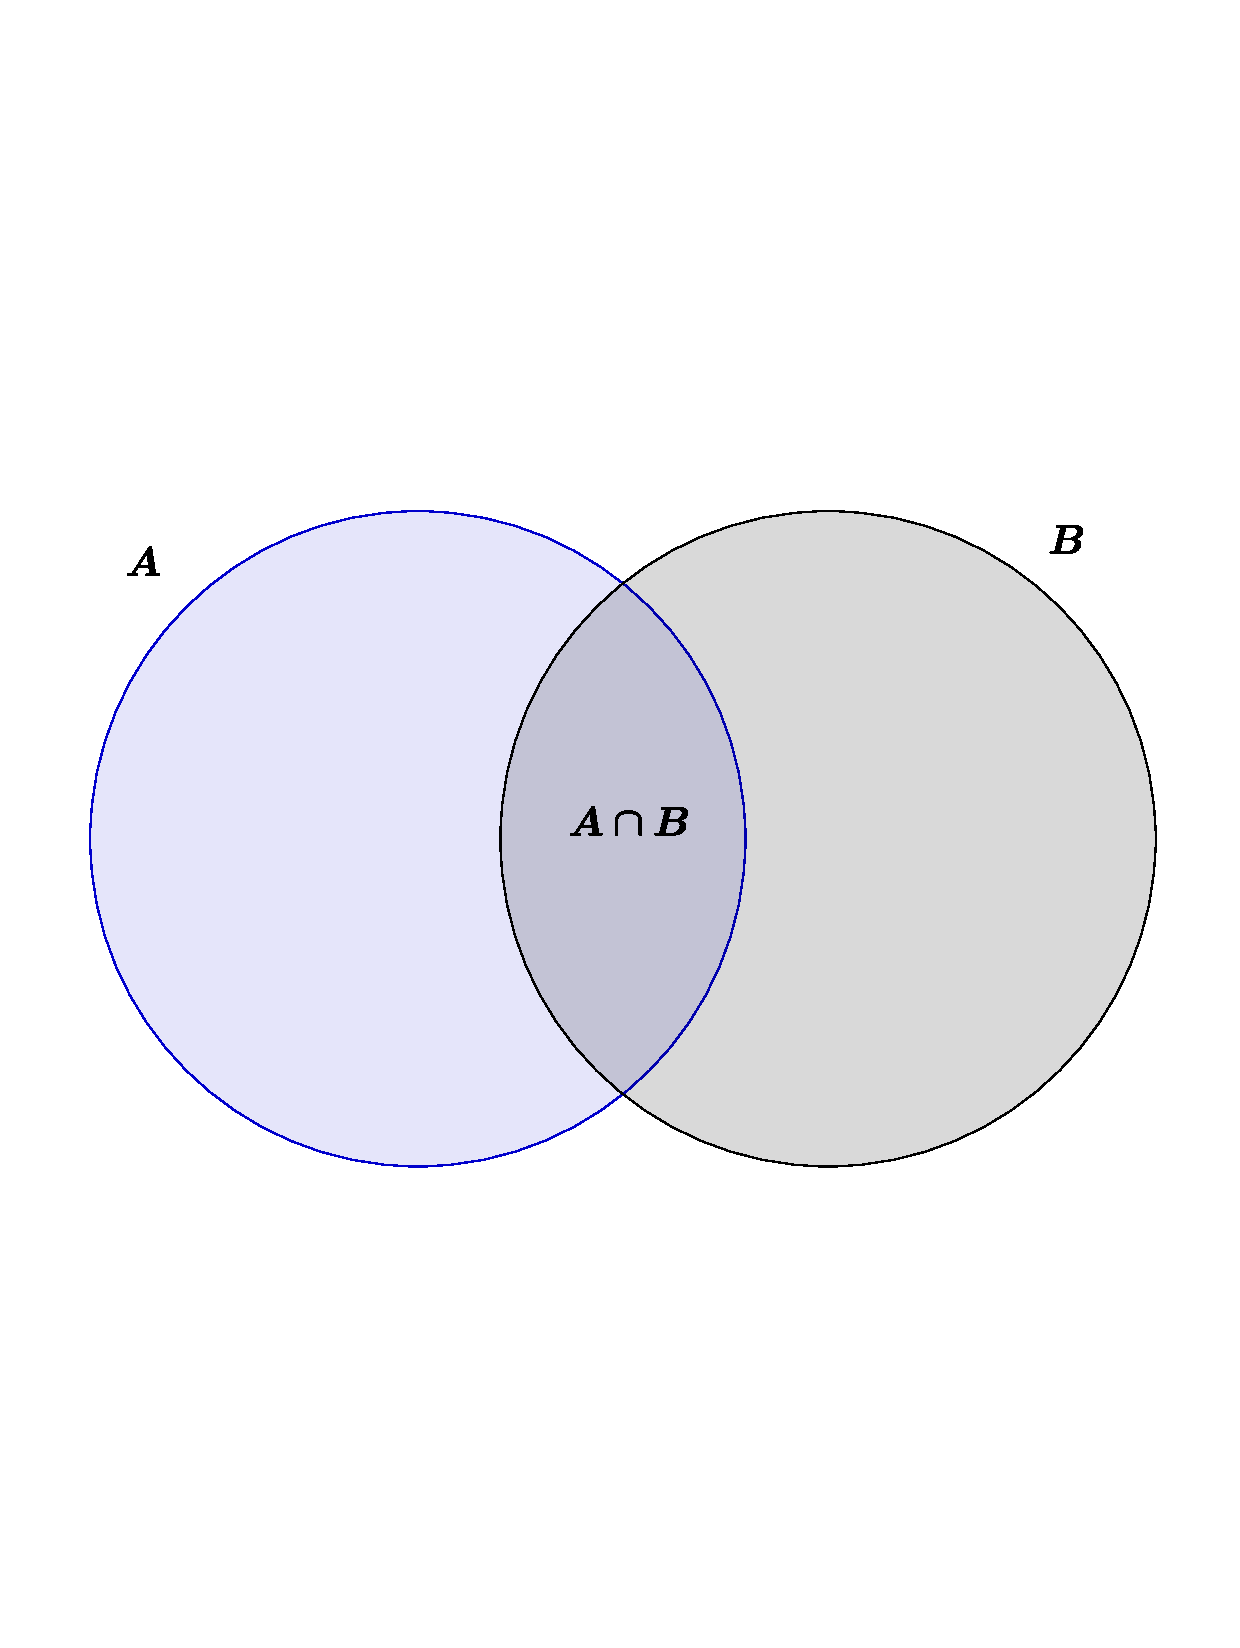
\includegraphics[scale=0.5]{figs/venn.pdf} 
    \caption{Provide a short caption description.}
    \label{fig:number}
 \end{figure}
 
 
% ----------------------------- %
% Tables
% ----------------------------- %
\subsection*{Tables}
We use the \texttt{booktabs} package.  Tables should present new information rather than duplicating what is in the text. Readers should be able to interpret the table without reference to the text. Please supply editable files.


\begin{table}[ht!]
\begin{center}
\begin{tabular}{lccc} 
	\toprule
	Date & Time  &  Average   & Standard Deviation \\ 
	\midrule
	Jan 1  & 1100	& 4.7		& 0.6		\\
	Jan 2  & 2300	& 16.7	& 2.9		\\
	Jan 3  & 1400	& 11.4	& 3.5		\\
	Jan 4  & 1130	& 8.4		& 2.1		\\
	Jan 5  & 500	& 5.2		& 1.9		\\
	Jan 6  & 1700	& 7.9		& 2.2		\\
	\bottomrule 
\end{tabular} 
\caption{This is a caption to the table}
\label{tab:1} 
\end{center}
\end{table} % end the table